\documentclass[10pt]{beamer}
\usetheme{metropolis}

\usepackage{tikz}
\usetikzlibrary{arrows.meta, positioning, shapes.geometric}
\usepackage{booktabs}
\usepackage{amsmath}

% ── Node colours ─────────────────────────────────────────────────────────────
\definecolor{planetcol}{HTML}{AED6F1}   % light blue
\definecolor{attackcol}{HTML}{FAD7A0}   % orange
\definecolor{stepcol} {HTML}{D5D8DC}   % grey
\definecolor{mastercol}{HTML}{A9DFBF}   % light green
\definecolor{basecol} {HTML}{EBF5FB}   % very pale blue (static base planet)

% ── Shared TikZ styles ───────────────────────────────────────────────────────
\tikzset{
  pnode/.style={circle, draw, fill=planetcol,  minimum size=0.75cm, font=\scriptsize, inner sep=1pt},
  anode/.style={circle, draw, fill=attackcol,  minimum size=0.65cm, font=\scriptsize, inner sep=1pt},
  snode/.style={rectangle, draw, fill=stepcol, minimum size=0.65cm, font=\scriptsize, inner sep=2pt},
  mnode/.style={diamond,   draw, fill=mastercol,minimum size=0.75cm, font=\scriptsize, inner sep=1pt},
  bnode/.style={circle, draw, fill=basecol,    minimum size=0.75cm, font=\scriptsize, inner sep=1pt, densely dashed},
  tnode/.style={circle, draw, fill=planetcol,  minimum size=0.75cm, font=\scriptsize, inner sep=1pt},
}

\title{GNN Modelisations for Orbit Wars}
\subtitle{Six graph representations for fleet decision-making}
\date{2026-06-07}
\author{}

\begin{document}
\maketitle

% ── Slide 2 : TOC ─────────────────────────────────────────────────────────────
\begin{frame}{Overview}
\begin{enumerate}
  \item \textbf{M1 — Edge prediction:} attacks as directed edges on planet graph
  \item \textbf{M2 — Hetero attack nodes:} tripartite planet\,$\to$\,attack\,$\to$\,planet
  \item \textbf{M3 — Attack-only graph:} attack nodes + same-src / same-dst edges
  \item \textbf{M4 — Step nodes:} ETA lifted into a dedicated node type
  \item \textbf{M5 — Temporal unrolling:} $N\times10$ planet copies across time
  \item \textbf{M6 — Hybrid bipartite:} base $+$ temporal snapshot $+$ attack nodes
\end{enumerate}

\vspace{6pt}
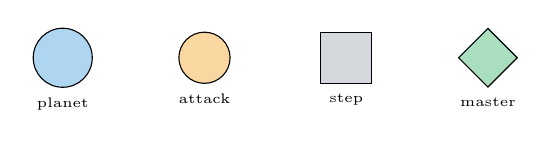
\begin{tikzpicture}[font=\tiny, >=Stealth]
  \node[pnode,  label=below:planet]  at (0,0)   {};
  \node[anode,  label=below:attack]  at (1.8,0) {};
  \node[snode,  label=below:step]    at (3.6,0) {};
  \node[mnode,  label=below:master]  at (5.4,0) {};
\end{tikzpicture}
\end{frame}

% ── Slide 3 : M1 ──────────────────────────────────────────────────────────────
\begin{frame}{M1 — Edge Prediction on Planet Graph}
\begin{columns}[T]

\begin{column}{0.44\textwidth}
\centering
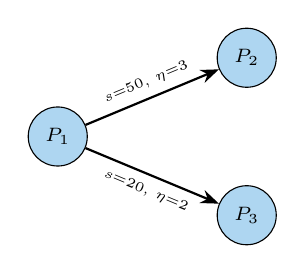
\begin{tikzpicture}[>=Stealth, font=\tiny]
  \node[pnode] (P1) at (0,   1.4) {$P_1$};
  \node[pnode] (P2) at (2.4, 2.4) {$P_2$};
  \node[pnode] (P3) at (2.4, 0.4) {$P_3$};
  \draw[->, thick] (P1) -- node[above,sloped]{$s{=}50,\,\eta{=}3$} (P2);
  \draw[->, thick] (P1) -- node[below,sloped]{$s{=}20,\,\eta{=}2$} (P3);
\end{tikzpicture}
\end{column}

\begin{column}{0.54\textwidth}
\footnotesize
\begin{tabular}{@{}p{1.7cm}p{3.5cm}@{}}
  \toprule
  Type & Features \\
  \midrule
  Planet node \newline (22-dim) &
    $x/100$,\,$y/100$,\,nature$^\dagger$,\,$\mathrm{prod}/5$,\,owner$^{\dagger\dagger}$,\,
    $\bigl[\tfrac{\log s_t}{\log 1024}\bigr]_{t=0}^{10}$ \\[6pt]
  Attack edge \newline (3-dim) &
    $\tfrac{\log s_{\min}}{\log 1024}$,\,$\tfrac{\log s_{\max}}{\log 1024}$,\,$\eta/9$ \\
  \bottomrule
\end{tabular}

\vspace{3pt}
{\tiny $^\dagger$fix/moving/comet (3 one-hot)\\
$^{\dagger\dagger}$neutral + 4 players (5 one-hot)}

\vspace{8pt}
\textbf{Task:} multi-label edge classification
\end{column}

\end{columns}
\end{frame}

% ── Slide 4 : M2 ──────────────────────────────────────────────────────────────
\begin{frame}{M2 — Heterogeneous Attack Nodes}
\begin{columns}[T]

\begin{column}{0.44\textwidth}
\centering
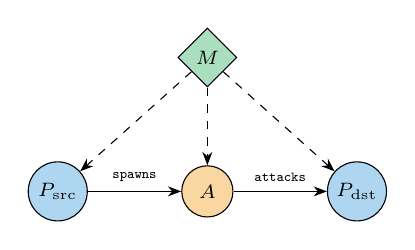
\begin{tikzpicture}[>=Stealth, font=\tiny]
  \node[pnode] (Ps) at (0,   1.2) {$P_{\text{src}}$};
  \node[anode] (A)  at (1.9, 1.2) {$A$};
  \node[pnode] (Pd) at (3.8, 1.2) {$P_{\text{dst}}$};
  \node[mnode] (M)  at (1.9, 2.9) {$M$};
  \draw[->] (Ps) -- node[above]{\texttt{spawns}}  (A);
  \draw[->] (A)  -- node[above]{\texttt{attacks}} (Pd);
  \draw[->, dashed] (M) -- (Ps);
  \draw[->, dashed] (M) -- (A);
  \draw[->, dashed] (M) -- (Pd);
\end{tikzpicture}
\end{column}

\begin{column}{0.54\textwidth}
\footnotesize
\begin{tabular}{@{}p{1.7cm}p{3.5cm}@{}}
  \toprule
  Type & Features \\
  \midrule
  Planet (22-dim) & same as M1 \\[4pt]
  Attack node \newline (3-dim) &
    $\tfrac{\log s_{\min}}{\log 1024}$,\,$\tfrac{\log s_{\max}}{\log 1024}$,\,$\eta/9$ \\[4pt]
  Master (6-dim) &
    $\mathrm{step}/500$,\,$\tfrac{\omega-0.025}{0.025}$,\,
    ship-prop $\times4$ \\
  \bottomrule
\end{tabular}

\vspace{6pt}
\textit{Matches \texttt{97-library.py} \texttt{build\_hetero\_data\_97}.}

\vspace{6pt}
\textbf{Task:} node classification on attack nodes
\end{column}

\end{columns}
\end{frame}

% ── Slide 5 : M3 ──────────────────────────────────────────────────────────────
\begin{frame}{M3 — Attack-Only Graph}
\begin{columns}[T]

\begin{column}{0.44\textwidth}
\centering
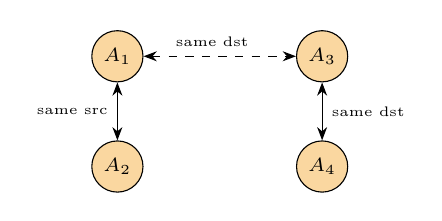
\begin{tikzpicture}[>=Stealth, font=\tiny]
  % left pair: same src
  \node[anode] (A1) at (0,   2.0) {$A_1$};
  \node[anode] (A2) at (0,   0.6) {$A_2$};
  % right pair: same dst
  \node[anode] (A3) at (2.6, 2.0) {$A_3$};
  \node[anode] (A4) at (2.6, 0.6) {$A_4$};
  \draw[<->] (A1) -- node[left] {same src} (A2);
  \draw[<->] (A3) -- node[right]{same dst} (A4);
  \draw[<->, dashed] (A1) -- node[above,sloped,pos=0.45]{same dst} (A3);
\end{tikzpicture}
\end{column}

\begin{column}{0.54\textwidth}
\footnotesize
\begin{tabular}{@{}p{1.9cm}p{3.3cm}@{}}
  \toprule
  Type & Features \\
  \midrule
  Attack node \newline (3-dim) &
    $\tfrac{\log s_{\min}}{\log 1024}$,\,$\tfrac{\log s_{\max}}{\log 1024}$,\,$\eta/9$ \\[4pt]
  Same-src edge & attacks from the same source planet \\[4pt]
  Same-dst edge & attacks targeting the same planet \\
  \bottomrule
\end{tabular}

\vspace{6pt}
No planet nodes — pure attack graph.

\vspace{6pt}
\textbf{Task:} node classification on attack nodes
\end{column}

\end{columns}
\end{frame}

% ── Slide 6 : M4 ──────────────────────────────────────────────────────────────
\begin{frame}{M4 — Step Nodes (ETA as Structure)}
\begin{columns}[T]

\begin{column}{0.44\textwidth}
\centering
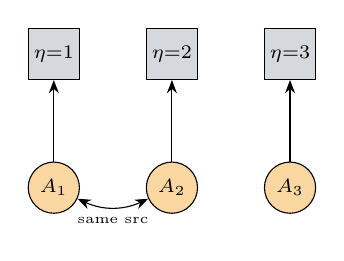
\begin{tikzpicture}[>=Stealth, font=\tiny]
  \node[snode] (S1) at (0,   2.7) {$\eta{=}1$};
  \node[snode] (S2) at (1.5, 2.7) {$\eta{=}2$};
  \node[snode] (S3) at (3.0, 2.7) {$\eta{=}3$};
  \node[anode] (A1) at (0,   1.0) {$A_1$};
  \node[anode] (A2) at (1.5, 1.0) {$A_2$};
  \node[anode] (A3) at (3.0, 1.0) {$A_3$};
  \draw[->] (A1) -- (S1);
  \draw[->] (A2) -- (S2);
  \draw[->] (A3) -- (S3);
  \draw[<->] (A1) to[bend right=25] node[below]{\tiny same src} (A2);
\end{tikzpicture}
\end{column}

\begin{column}{0.54\textwidth}
\footnotesize
\begin{tabular}{@{}p{1.9cm}p{3.3cm}@{}}
  \toprule
  Type & Features \\
  \midrule
  Attack node \newline (2-dim) &
    $\tfrac{\log s_{\min}}{\log 1024}$,\,$\tfrac{\log s_{\max}}{\log 1024}$ \\[4pt]
  Step node \newline (0-dim) & no features; identity = ETA \\[4pt]
  Attack\,$\to$\,Step & connects attack to its ETA bucket \\[4pt]
  Same-src/dst & same as M3 \\
  \bottomrule
\end{tabular}

\vspace{6pt}
ETA is structural, not a feature.

\vspace{6pt}
\textbf{Task:} node classification on attack nodes
\end{column}

\end{columns}
\end{frame}

% ── Slide 7 : M5 ──────────────────────────────────────────────────────────────
\begin{frame}{M5 — Temporal Unrolling}
\begin{columns}[T]

\begin{column}{0.44\textwidth}
\centering
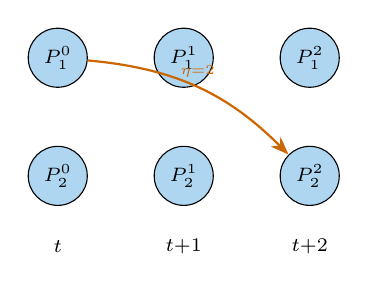
\begin{tikzpicture}[>=Stealth, font=\tiny]
  \node[pnode] (P10) at (0,   2.5) {$P_1^0$};
  \node[pnode] (P20) at (0,   1.0) {$P_2^0$};
  \node[pnode] (P11) at (1.6, 2.5) {$P_1^1$};
  \node[pnode] (P21) at (1.6, 1.0) {$P_2^1$};
  \node[pnode] (P12) at (3.2, 2.5) {$P_1^2$};
  \node[pnode] (P22) at (3.2, 1.0) {$P_2^2$};
  % cross-time attack edge: P1[t=0] -> P2[t=2], ETA=2
  \draw[->, thick, orange!80!black]
    (P10) to[bend left=20] node[above,pos=0.5]{$\eta{=}2$} (P22);
  % time labels
  \foreach \x/\t in {0/t, 1.6/{t{+}1}, 3.2/{t{+}2}}
    \node[font=\scriptsize] at (\x, 0.1) {$\t$};
\end{tikzpicture}
\end{column}

\begin{column}{0.54\textwidth}
\footnotesize
\begin{tabular}{@{}p{1.9cm}p{3.3cm}@{}}
  \toprule
  Type & Features \\
  \midrule
  Planet$^t$ node \newline (12-dim) &
    $x^t/100$,\,$y^t/100$,\,nature$^\dagger$,\,$\mathrm{prod}/5$,\,
    owner$^{\dagger\dagger}$,\,$\tfrac{\log s^t}{\log 1024}$ \\[6pt]
  Attack edge \newline (1-dim) &
    $\tfrac{\log s_{\min}}{\log 1024}$ \\
  \bottomrule
\end{tabular}

\vspace{3pt}
{\tiny $^\dagger$fix/moving/comet \hfill $^{\dagger\dagger}$5-class one-hot}

\vspace{5pt}
$P_{\text{src}}^{t=i}\;\xrightarrow{\;\eta\;}\;P_{\text{dst}}^{t=i+\eta}$\\[3pt]
$N\times10$ planet nodes total.

\vspace{6pt}
\textbf{Task:} multi-label edge classification
\end{column}

\end{columns}
\end{frame}

% ── Slide 8 : M6 ─────────────────────────────────────────────────────────────
\begin{frame}{M6 — Hybrid Bipartite Action-Selector}
\begin{columns}[T]

\begin{column}{0.50\textwidth}
\centering
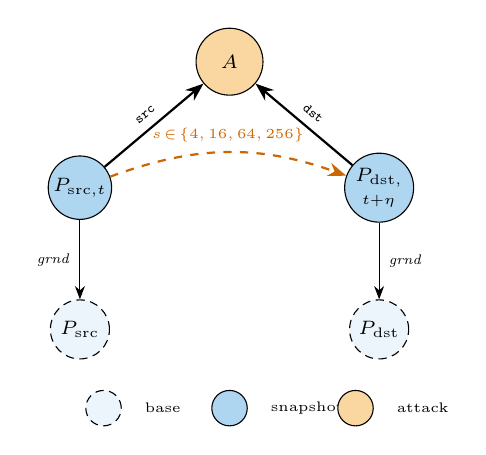
\begin{tikzpicture}[>=Stealth, font=\tiny, node distance=0pt]
  % ── base planet nodes (foundation, pale dashed) ──────────────────
  \node[bnode] (Pb_s) at (-1.9, 0.0) {$P_{\text{src}}$};
  \node[bnode] (Pb_d) at ( 1.9, 0.0) {$P_{\text{dst}}$};
  % ── temporal snapshot nodes (middle row) ─────────────────────────
  \node[tnode] (Pt_s) at (-1.9, 1.8) {$P_{\text{src},t}$};
  \node[tnode] (Pt_d) at ( 1.9, 1.8) {\shortstack{$P_{\text{dst},}$\\$_{t+\eta}$}};
  % ── attack node (top centre) ─────────────────────────────────────
  \node[anode, minimum size=0.85cm] (A) at (0, 3.4) {$A$};
  % ── state-to-base ────────────────────────────────────────────────
  \draw[->] (Pt_s) -- node[left, pos=0.5]{\textit{grnd}} (Pb_s);
  \draw[->] (Pt_d) -- node[right,pos=0.5]{\textit{grnd}} (Pb_d);
  % ── attack-action edges ──────────────────────────────────────────
  \draw[->, thick] (Pt_s) -- node[above,sloped]{\texttt{src}} (A);
  \draw[->, thick] (Pt_d) -- node[above,sloped]{\texttt{dst}} (A);
  % ── temporal attack edge (dashed, discrete ships) ─────────────────
  \draw[->, dashed, orange!80!black, thick]
    (Pt_s) to[bend left=20]
    node[above, pos=0.5]{$s\!\in\!\{4,16,64,256\}$} (Pt_d);
  % ── legend strip ─────────────────────────────────────────────────
  \node[bnode, minimum size=0.45cm, font=\tiny] at (-1.6,-1.0) {};
  \node[font=\tiny, anchor=west] at (-1.2,-1.0) {base};
  \node[tnode, minimum size=0.45cm, font=\tiny] at ( 0.0,-1.0) {};
  \node[font=\tiny, anchor=west] at ( 0.4,-1.0) {snapshot};
  \node[anode, minimum size=0.45cm, font=\tiny] at ( 1.6,-1.0) {};
  \node[font=\tiny, anchor=west] at ( 2.0,-1.0) {attack};
\end{tikzpicture}
\end{column}

\begin{column}{0.48\textwidth}
\footnotesize
\begin{tabular}{@{}p{1.7cm}p{3.3cm}@{}}
  \toprule
  Type & Features \\
  \midrule
  Base $P_i$ \newline (4-dim) &
    nature$^\dagger$ (one-hot),\,$\mathrm{prod}/5$ \\[4pt]
  Snapshot $P_{i,t}$ \newline (9-dim) &
    $x/100$,\,$y/100$,\,$\tfrac{\log s}{\log 1024}$,\,
    owner$^{\dagger\dagger}$ (one-hot),\,$t/20$ \\[4pt]
  Attack $A$ \newline (1-dim) &
    $\tfrac{\log s_{\text{fleet}}}{\log 1024}$ \\
  \bottomrule
\end{tabular}

\vspace{4pt}
{\tiny $^\dagger$fix/moving/comet \hfill $^{\dagger\dagger}$5-class one-hot}

\vspace{5pt}
\textbf{Edges:}
\begin{itemize}\scriptsize
  \item $P_{i,t}\!\to\!P_i$ \ state-to-base (grounding)
  \item $P_{\text{src},t}\!\to\!A$,\,$P_{\text{dst},t+\eta}\!\to\!A$ \ attack-action
  \item $P_{i,t_i}\!\dashrightarrow\!P_{j,t_j}$ \ temporal ($s\!\in\!\{4,16,64,256\}$)
\end{itemize}

\vspace{5pt}
\textbf{Task:} node classification on attack nodes
\end{column}

\end{columns}
\end{frame}

% ── Slide 9 : Add-ons ─────────────────────────────────────────────────────────
\begin{frame}{Add-ons / Extensions}
Applicable to any modelisation:

\begin{itemize}
  \item \textbf{Master node} — global context, connected to all planet/attack nodes
  \begin{itemize}\small
    \item $\mathrm{step}/500$,\quad $(\omega-0.025)/0.025$,\quad ship-proportion $\times4$ players
  \end{itemize}

  \vspace{4pt}
  \item \textbf{Comet-aware features} — comet flag in nature one-hot; optionally add path index

  \vspace{4pt}
  \item \textbf{Lookahead labels} — label attacks by forward-simulated $\Delta\mathrm{ships}$ instead of heuristic selection

  \vspace{4pt}
  \item \textbf{Fleet nodes} — in-flight fleets as explicit nodes:
        $x,\,y,\,\mathrm{angle},\,s,\,\mathrm{ETA}_{\text{each planet}}$
\end{itemize}
\end{frame}

\end{document}
